\documentclass{report}
\usepackage{graphicx}
\usepackage{booktabs}
\usepackage[Export]{adjustbox}
\usepackage{pgf-pie}
\usepackage{hyperref}
\usepackage{enumitem}
\usepackage{amsmath}
\usepackage[makeroom]{cancel}
\usepackage{xcolor}
\usepackage{titlesec}
\usepackage{chngcntr}
\usepackage{accents}
\usepackage{pgfplots}
\usepackage{setspace}
\usepackage{tikz}
\usetikzlibrary{tikzmark}
\usetikzlibrary{arrows}
\usetikzlibrary{matrix}
\pgfplotsset{compat=1.18}

\hypersetup{
    colorlinks=true,
    linkcolor=blue,
    filecolor=magenta,      
    urlcolor=cyan,
    pdftitle={Latihan Soal PSAJ Matematika},
    pdfpagemode=FullScreen,
    }
\urlstyle{same}

\newcommand{\options}[5]{
\begin{enumerate}[label=\alph*.]
	\item #1
	\item #2
	\item #3
	\item #4
	\item #5
\end{enumerate}
}


\newcommand{\pemb}{ \textbf{Pembahasan} \\}


\titleformat{\chapter}[display]
  {\normalfont\bfseries}{}{0pt}{\Large}

\counterwithin*{equation}{section}
\counterwithin*{equation}{chapter}

\begin{document}


\begin{enumerate}
% No. 1
\item
Bentuk sederhana dari $\left(\frac{x^{2}y^{3}z^{-1}}{x^{-3}y^{-4}z^{3}}\right)^3$ adalah \ldots
\options
{$\frac{x^{15} y^{21}}{z^6}$}
{$\frac{x^{15} y^{21}}{z^8}$}
{\textcolor{red}{{$\frac{x^{15} y^{21}}{z^{12}}$}}}
{$\frac{x^{15} y^{21}}{z^{10}}$}
{$\frac{x^{15} y^{21}}{z^{14}}$}

\pemb

\begin{align*}
	\left(\frac{x^{2}y^{3}z^{-1}}{x^{-3}y^{-4}z^{3}}\right)^3 
	&= \frac{x^{6}y^{9}z^{-3}}{x^{-9}y^{-12}z^{9}} \\
	&= \frac{x^{6}y^{9}x^{9}y^{12}}{z^{3}z^{9}} \\
	&= \frac{x^{15} y^{21}}{z^{12}} \text{(C)}
\end{align*}
% No. 2
\item
Nilai dari $\left(\frac{1}{8}\right)^{\frac{-2}{3}}+32^{\frac{2}{5}}+27^{\frac{2}{3}}$ adalah \ldots
\options
{8}
{9}
{10}
{14}
{\textcolor{red}{17}}

\pemb
\begin{align*}
	\left(\frac{1}{8}\right)^{\frac{-2}{3}}+32^{\frac{2}{5}}+27^{\frac{2}{3}} 
	&= \sqrt[3]{\left(\frac{1}{8}\right)^{-2}}+\sqrt[5]{32^{2}}+\sqrt[3]{27^{2}} \\
	&= \sqrt[3]{\frac{1^{-2}}{8^{-2}}}+\sqrt[5]{32^{2}}+\sqrt[3]{27^{2}} \\
	&= \sqrt[3]{\frac{\frac{1}{1^{2}}}{\frac{1}{8^{2}}}}+\sqrt[5]{32^{2}}+\sqrt[3]{27^{2}}\\
	&= \sqrt[3]{64}+\sqrt[5]{32^{2}}+\sqrt[3]{27^{2}}\\
	&= 4 + 2^2 + 3^2 \\
	&= 4 + 4 + 9 \\
	&= 17  \text{(E)}
\end{align*}

% No. 3
\item
Hasil dari $2\sqrt{48}-4\sqrt{75}+3\sqrt{12}$ = \ldots
\options
{$18\sqrt{3}$}
{$12\sqrt{3}$}
{$3\sqrt{3}$}
{$-3\sqrt{3}$}
{\textcolor{red}{$-6\sqrt{3}$}}
\pemb
Karena semua pilihan memiliki $\sqrt{3}$, maka akar-akar disederhanakan ke bentuk $x\sqrt{3}$
\begin{align*}
	2\sqrt{48}-4\sqrt{75}+3\sqrt{12} 
	&= 2\sqrt{16.3}-4\sqrt{25.3}+3\sqrt{4.3} \\
	&= 2.4\sqrt{3}-4.5\sqrt{3}+3.2\sqrt{3} \\
	&= 8\sqrt{3}-20\sqrt{3}+6\sqrt{3} \\
	&= -6\sqrt{3} \text{(E)}
\end{align*}

% No. 4
\item
Bentuk sederhana dari $\frac{3\sqrt{5}}{3\sqrt{5}+\sqrt{3}}$ adalah \ldots
\options
{$\frac{15-\sqrt{15}}{-14}$}
{$\frac{15+\sqrt{15}}{-14}$}
{\textcolor{red}{$\frac{15-\sqrt{15}}{14}$}}
{$\frac{12-\sqrt{15}}{-14}$}
{$\frac{12-\sqrt{15}}{15}$}
\pemb
Rasionalkan akar dengan cara mengalikan pembilang dan penyebut dengan pasangan sekawan dari penyebut
\begin{align*}
	\frac{3\sqrt{5}}{3\sqrt{5}+\sqrt{3}} \cdot \frac{3\sqrt{5}-\sqrt{3}}{3\sqrt{5}-\sqrt{3}}
	&= \frac{3\sqrt{5}\left(3\sqrt{5}-\sqrt{3}\right)}{45-3} \\
	&= \frac{\cancel{3}\sqrt{5}\left(3\sqrt{5}-\sqrt{3}\right)}{\cancelto{14}{42}} \\
	&= \frac{\sqrt{5}\left(3\sqrt{5}-\sqrt{3}\right)}{14} \\
	&= \frac{3.5-\sqrt{15}}{14} \\
	&= \frac{15-\sqrt{15}}{14} \text{(C)}
\end{align*}

% No. 5
\item
Nilai dari ${}^{16}\log_{81}.{}^{3}\log_{125}.{}^{5}\log_{32}$ adalah \ldots
\options
{8}
{10}
{\textcolor{red}{15}}
{28}
{32}
\pemb
\begin{align*}
	{}^{16}\log_{81}.{}^{3}\log_{125}.{}^{5}\log_{32} 
	&= {}^{2^{4}}\log_{3^{4}}.{}^{3^1}\log_{5^3}.{}^{5^1}\log_{2^5} \\
	&= \frac{4}{4}\cdot\frac{3}{1}\cdot\frac{5}{1}{}^{2}\log_{3}.{}^{3}\log_{5}.{}^{5}\log_{2} \\
	&= 15 {}^{2}\log_{2} \\
	&= 15.1 \\
	&= 15 \text{(C)}
\end{align*}

\item
Nilai dari ${}^{3}\log_{81}+{}^{5}\log_{300}-{}^{5}\log_{12}+{}^{2}\log_{\frac{1}{64}}$ adalah \ldots
\options
{-2}
{-1}
{\textcolor{red}0}
{1}
{6}
\pemb
\begin{align*}
	{}^{3}\log_{81}+{}^{5}\log_{300}-{}^{5}\log_{12}+{}^{2}\log_{\frac{1}{64}} 
	&= {}^{3}\log_{81}+{}^{5}\log_{\frac{300}{12}}+{}^{2}\log_{\frac{1}{64}} \\
	&= {}^{3}\log_{81}+{}^{5}\log_{25}+{}^{2}\log_{\frac{1}{64}} \\
	&= {}^{3}\log_{3^4}+{}^{5}\log_{5^2}+{}^{2}\log_{2^{-6}} \\
	&= 4 + 2 - 6 \\
	&= 0 \text{(C)}
\end{align*}

% No. 7
\item
Akar -akar penyelesaian persamaan kuadrat $x^2-x-20=0$ adalah \ldots
\options
{-4 dan -5}
{4 dan -5}
{\textcolor{red}{-4 dan 5}}
{2 dan -10}
{2 dan 10}
\pemb
Faktorkan Persamaan Kuadrat
\begin{align*}
    x^2-x-20&=0 \\
    (x+4)(x-5)&=0
\end{align*}
\begin{center}
\begin{tabular}{c c c}
	\parbox{3cm}{
		\begin{align*}
		x+4&=0 \\
		x&=-4
		\end{align*}
	} & \parbox{0.8cm}{atau} &
	\parbox{3cm}{
		\begin{align*}
		x-5&=0 \\
		x&=5
		\end{align*}
	}
\text{(C)}
\end{tabular}
\end{center}

% No. 8
\item Perhatikan grafik berikut! \\
\begin{tikzpicture}
	\begin{axis}[ymin=-10, ymax=10, xmin=-10, xmax=10,
		axis line style={->},
		axis lines=middle,
		xlabel=$x$,
		ylabel=$y$,
		domain=-1:7
		]
	\addplot+[<->,mark=none,line width=1pt, samples=100]{x^2-6*x+5};
	\addplot [blue, mark = *, nodes near coords=\textcolor{black}{(3, -4)},every node near coord/.style={anchor=90}] coordinates {(3,-4)};
	\end{axis}
\end{tikzpicture}
Persamaan grafik fungsi kuadrat tersebut adalah \ldots
\options
{$y = x^2-5x+6$}
{$y = x^2-6x+5$}
{$y = x^2+6x-5$}
{$y = x^2-5x-6$}
{\textcolor{red}{$y = x^2-6x+5$}}
\pemb
Graf tersebut berpotongan dengan sumbu x pada titik \text{(1, 0)} dan \text{(5, 0)}
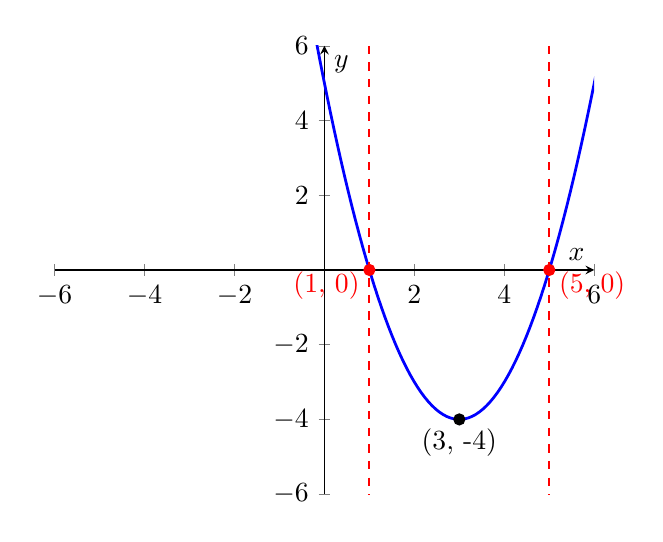
\begin{tikzpicture}
	\begin{axis}[ymin=-6, ymax=6, xmin=-6, xmax=6,
		axis line style={->},
		axis lines=center,
		xlabel=$x$,
		ylabel=$y$,
		domain=-1:7
		]
	\addplot+[<->,mark=none,line width=1pt, samples=100]{x^2-6*x+5};
	\addplot [black, mark = *, nodes near coords=\text{(3, -4)},every node near coord/.style={anchor=90}] coordinates {(3,-4)};
	\addplot[thick, samples=50, dashed,red] coordinates {(5,10)(5,-15)};
	\addplot [red, mark = *, nodes near coords=\text{(5, 0)},every node near coord/.style={anchor=160}] coordinates {(5, 0)};
	\addplot[thick, samples=50, dashed,red] coordinates {(1,10)(1,-15)};
	\addplot [red, mark = *, nodes near coords=\text{(1, 0)},every node near coord/.style={anchor=20}] coordinates {(1, 0)};
	\end{axis}
\end{tikzpicture}
\[
	x_{1} = 1 \text{ dan } x_{2} = 5
\]
Mencari persamaan kuadrat
\begin{align*}
	y 
	&= (x-x_{1})(x-x_{2}) \\
	&= (x-1)(x-5) \\
	&= x^2-6x+5 \text{ (E)}
\end{align*}

% No. 9
\item Persamaan kuadrat $2x^2-4x+7=0$ mempunyai akar-akar $x_{1}$ dan $x_{2}$. Persamaan kuadrat yang akar-akarnya $x_{1} - 2$ dan $x_{2} - 2$ adalah \ldots
\options
{$-2x^2-4x+7=0$}
{$2x^2-4x+7=0$}
{\textcolor{red}{$2x^2+4x+7=0$}}
{$2x^2-4x-7=0$}
{$2x^2+4x-7=0$}
\pemb
Persamaan kuadrat yang akar-akarnya \emph{k} lebihnya dari ($x_{1}+k$) dan ($x_{2}+k$) akar-akar persamaan $ax^2+bx+c=0$ adalah $a(x-k)^2+b(x-k)+c=0$
\begin{align*}
	2(x+2)^2-4(x+2)+7 &= 0 \\
	2(x^2+4x+4)-4x-8+7 &= 0 \\
	2x^2+8x+8-4x-8+7 &= 0 \\
	2x^2+4x+7 &= 0 \\
\end{align*}
\end{enumerate}

\begin{enumerate}
\setcounter{enumi}{7}
% No. 8
\item Jika persamaan $x_{1}$ dan $x_{2}$ merupakan akar-akar persamaan $x^2+2x-5=0$, persamaan kuadrat baru yang mempunyai akar-akar $2x_{1}$ dan $2x_{2}$ adalah \ldots
\options
{$x^2-2x+10=0$}
{$x^2+2x-10=0$}
{$x^2+4x-10=0$}
{$x^2-4x+20=0$}
{\textcolor{red}{$x^2+4x-20=0$}}
\pemb
Persamaan kuadrat yang akar-akarnya \emph{n} kali (artinya : $nx_{1}$ dan $nx_{2}$) akar-akar persamaan $ax^2+bx+c=0$ adalah $ax^2+n.bx+n^2.c=0$
\begin{align*}
	x^2+2x-5 &= 0 \\
	x^2+2(2)x-5(2^2) &= 0 \\
	x^2+4x-20 &= 0 \\
\end{align*}

% No. 9
\item Jika persamaan $x_{1}$ dan $x_{2}$ merupakan akar-akar persamaan $x^2+2x-5=0$, persamaan kuadrat baru yang mempunyai akar-akar $2x_{1}$ dan $2x_{2}$ adalah \ldots
\options
{$x^2-2x+10=0$}
{$x^2+2x-10=0$}
{$x^2+4x-10=0$}
{$x^2-4x+20=0$}
{\textcolor{red}{$x^2+4x-20=0$}}
\pemb
Persamaan kuadrat yang akar-akarnya \emph{n} kali (artinya : $nx_{1}$ dan $nx_{2}$) akar-akar persamaan $ax^2+bx+c=0$ adalah $ax^2+n.bx+n^2.c=0$
\begin{align*}
	x^2+2x-5 &= 0 \\
	x^2+2(2)x-5(2^2) &= 0 \\
	x^2+4x-20 &= 0 \\
\end{align*}

% No. 10
\item Diketahui matriks $ P=
	\begin{bmatrix}
		x+2y & 3 \\
		2x-y & -6 \\
	\end{bmatrix}
	$  dan $Q=
	\begin{bmatrix}
		-4 & -3 \\
		3 & -6 \\
	\end{bmatrix}
	$. Jika $P^{T} = Q$ maka nilai $4x-3y$ adalah \ldots
	\options
	{-11}
	{\textcolor{red}{-5}}
	{-3}
	{5}
	{11}
	\pemb
	Transposisi matriks \\
	    A = $\begin{bmatrix}
			a & b & c\\
			d & e & f\\
		\end{bmatrix}
		\to
		A^{T} = \begin{bmatrix}
			a & d \\
			b & e \\
			c & f \\
		\end{bmatrix}$
	Maka
	\begin{align*}
		P^T 
		&= Q \\
		\begin{bmatrix}
			x+2y & 2x-y \\
			3 & -6 \\
		\end{bmatrix} &=
		\begin{bmatrix}
			-4 & -3 \\
			3 & -6 \\
		\end{bmatrix}
	\end{align*}
	Selesaikan persamaan linear dua variabel tersebut
	\begin{center}
	\begin{tabular}{c|c|c}
		\parbox{3cm}{
			\begin{align*}
			x+2y &= -4 \\
			2x-y &= -3
			\end{align*}
		} & \parbox{0.3cm}{
			-2 \\ 1 
		} &
		\parbox{3cm}{
			\begin{align*}
			-2x-4y&=8\\
			-2x-y&=-3
			\end{align*}
		} \\
		\cline{3-3}
	\end{tabular} 
	\begin{tabular}{c c c}
		\parbox{3cm}{\textcolor{white}{
			\begin{align*}
			x+2y &= -4 \\
			2x-y &= -3
			\end{align*}}
		} & \parbox{0.3cm}{\textcolor{white}{
			-2 \\ 1 }
		} &
		\parbox{3cm}{
			\begin{align*}
				-5y&=5\\
				y&=-1
			\end{align*}
		} \\
	\end{tabular}
	\end{center}
	Cari nilai \emph{x} melalui substitusi
	\begin{align*}
		x+2y&=-4\\
		x+2(-1)&=-4\\
		x-2&=-4\\
		x&=-2\\
	\end{align*}
	Maka nilai $4x-3y$ adalah \\
	\begin{align*}
	4x-3y&=4(-2)-3(-1)\\
	&=-8+3 \\
	&=-5 \text{(B)}
	\end{align*}

% No. 11
\item Diketahui matriks $P = 
\begin{bmatrix}
4 & 3 & 2 \\ 
-1 & 0 & 1 \\ 
-2 & -3 & - 4 \\
\end{bmatrix}
$. Determinan dari matriks P adalah \ldots
\options
{24}
{12}
{\textcolor{red}{0}}
{-12}
{-24}
\pemb
Determinan matriks 3x3 
\begin{align*}
    A = \begin{bmatrix}
		a & b & c \\
		d & e & f \\
		g & h & i \\
	\end{bmatrix}
	\to \text{det(A)} &= 
	\text{det}
		\begin{bmatrix}
			a & b & c \\
			d & e & f \\
			g & h & i \\
		\end{bmatrix} \\
	&= 
	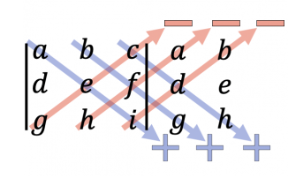
\includegraphics[valign=c,width=50mm,scale=0.5]{sarrus.png}\\
	&= (aei + bfg + cdh) - (ceg + afh + bdi)
\end{align*}
\begin{align*}
	\text{det}
	\begin{bmatrix}
		4 & 3 & 2 \\ 
		-1 & 0 & 1 \\ 
		-2 & -3 & - 4 \\
	\end{bmatrix} 
	&= (4.0.(-4)+3.1.(-2)+2.-1.(-3)) - (2.0.(-2)+4.1.(-3)+3.-1.(-4)) \\
	&= (0+(-6)+6) - (0+(-12)+12) \\
	&= 0 \text{( C)}
\end{align*}

% No. 12
\item Diketahui matriks $A = \begin{bmatrix}
	1 & 3 \\
	2 & -1 \\
	4 & 1 \\
\end{bmatrix}$ dan $B=\begin{bmatrix}
	3 & -2 \\
	2 & -1 \\
\end{bmatrix}$ hasil dari \emph{A x B} adalah\ldots
\options
{$
	\begin{bmatrix}
		9 & -5 \\
		4 & -3 \\
		14 & 9 \\
	\end{bmatrix}
$}
{$
	\begin{bmatrix}
		-9 & -5 \\
		4 & -3 \\
		14 & -9 \\
	\end{bmatrix}
$}
{\textcolor{red}{$
	\begin{bmatrix}
		9 & -5 \\
		4 & -3 \\
		14 & -9 \\
	\end{bmatrix}
$}}
{$
	\begin{bmatrix}
		9 & 5 \\
		4 & -3 \\
		14 & -9 \\
	\end{bmatrix}
$}
{$
	\begin{bmatrix}
		-9 & -5 \\
		4 & -3 \\
		14 & 9 \\
	\end{bmatrix}
$}
\pemb
Perkalian matriks 
$
	\begin{bmatrix}
		a & b \\
		c & d \\
		e & f \\
	\end{bmatrix} 
	\cdot
	\begin{bmatrix}
		g & h \\
		i & j \\
	\end{bmatrix} 
	=
	\begin{bmatrix}
		a.g + b.i & a.h + b.j\\
		c.g + d.i & c.h + d.j\\
		e.g + f.i & e.h + f.j\\
	\end{bmatrix}
$ \\
Maka 
\begin{align*}
\begin{bmatrix}
	1 & 3 \\
	2 & -1 \\
	4 & 1 \\
\end{bmatrix}
\cdot
\begin{bmatrix}
	3 & -2 \\
	2 & -1 \\
\end{bmatrix} 
	&= 
	\begin{bmatrix}
		1.3 + 3.2  & 1.-2 + 3(-1)\\
		2.3 + (-1)2 & 2.-2 + -1(-1)\\
		4.3 + 1.2  & 4.-2 + 1(-1)\\
	\end{bmatrix}
	\\
	&= 
	\begin{bmatrix}
		9 & -5\\
		4 & -3\\
		14 & -9\\
	\end{bmatrix} \text{ (C)}
\end{align*}

% No. 13
\item Diketahui matriks $A = \begin{bmatrix}
	5 & -8 \\
	4 & -6 \\
\end{bmatrix}$. Invers dari matriks A adalah
\options
{$
	\frac{1}{2} 
	\begin{bmatrix}
		-6 & -8 \\
		4 & -5 \\
	\end{bmatrix}
$}
{$
	\frac{1}{2} 
	\begin{bmatrix}
		-6 & 8 \\
		4 & 5 \\
	\end{bmatrix}
$}
{$
	\frac{1}{2} 
	\begin{bmatrix}
		-6 & -8 \\
		4 & 5 \\
	\end{bmatrix}
$}
{$
	\frac{1}{2} 
	\begin{bmatrix}
		-6 & 8 \\
		-4 & 5 \\
	\end{bmatrix}
$}
{$
	\frac{1}{2} 
	\begin{bmatrix}
		-6 & -8 \\
		-4 & 5 \\
	\end{bmatrix}
$}
\pemb
\begin{align*}
    A = \begin{bmatrix}
		a & b \\
		c & d \\
	\end{bmatrix}
	\to
	A^{-1} = 
	\frac{1}{ad-bc}
	\begin{bmatrix}
		d & -b \\
		-c & a \\
	\end{bmatrix}
\end{align*}
Maka 
\begin{align*}
	A^{-1}
	\begin{bmatrix}
		5 & -8 \\
		4 & -6 \\
	\end{bmatrix}
	&= \frac{1}{5(-6) - (-8)4} 
	\begin{bmatrix}
		6 & 8 \\
		-4 & 5 \\
	\end{bmatrix} \\
	&= -\frac{1}{2} 
	\begin{bmatrix}
		6 & 8 \\
		-4 & 5 \\
	\end{bmatrix}\\
	&= \frac{1}{2} 
	\begin{bmatrix}
		-6 & -8 \\
		4 & -5 \\
	\end{bmatrix} \text{ (A)}
\end{align*}

\item Seorang pembuat kue akan membuat dua jenis kue dengan bahan dasar yang sama. Kue
jenis I membutuhkan 200 gram terigu dan 300 gram mentega, sedangkan kue jenis
kedua membutuhkan 300 gram terigu dan 100 gram mentega . Jika persediaan terigu dan
mentega masing – masing hanya 1400 gram dan 1100 gram, model matematika
permasalahan di atas adalah \ldots
\options
{\textcolor{red}{$2x+3y\leq14;3x+y\leq11;x\geq0;y\geq0$}}
{$2x+3y\geq14;3x+y\leq11;x\geq0;y\geq0$}
{$2x+3y\leq14;3x+y\geq11;x\geq0;y\geq0$}
{$3x+2y\leq14;3x+y\leq11;x\geq0;y\geq0$}
{$2x+3y\leq14;x+3y\leq11;x\geq0;y\geq0$}
\pemb
\\
\begin{center}
\begin{tabular}{|c|c|c|c|}
	\hline
	Kue & Terigu & Mentega & Persediaan \\
	\hline
	Jenis I & $2\cancel{00}$ & $3\cancel{00}$ & $14\cancel{00}$ \\
	\hline
	Jenis II & $3\cancel{00}$ & $1\cancel{00}$ & $11\cancel{00}$ \\
	\hline
\end{tabular}
\end{center}
Karena jumlah terigu dan mentega yang digunakan tidak boleh melebihi persediaan maka pertidaksamaan ditandai dengan $\leq$

\item Perhatikan grafik sistem pertidaksamaan linier di bawah ini ! \\
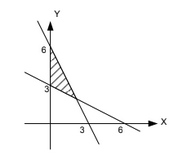
\includegraphics{graf_pertidak.png} \\
Daerah yang di arsir adalah daerah himpunan penyelesaian permasalahan program linear. Nilai maksimum dari fungsi obyektif $f(x,y) = 2x+3y$ adalah
\options
{9}
{10}
{14}
{\textcolor{red}{18}}
{20}
\pemb
Cari persamaan dari kedua garis\\
\begin{itemize}
	\item Garis pertama \\
	\begin{tikzpicture}
		\begin{axis}[ymin=-2,xmin=-2,ymax=7,xmax=7,axis lines=middle]
		\addplot[red]{-2*x+6};
		\end{axis}
	\end{tikzpicture}
	\begin{align*}
		m&=\frac{6-0}{0-3}\\
		&=-2\\
		y&=-2x+6\\
	\end{align*}
	\item Garis kedua \\
	\begin{tikzpicture}
		\begin{axis}[ymin=-2,xmin=-2,ymax=7,xmax=7,axis lines=middle,domain=-1:7]
		\addplot[red]{-0.5*x+3};
		\end{axis}
	\end{tikzpicture}
	\begin{align*}
		m&=\frac{3-0}{0-6}\\
		&=-2\\
		y&=-\frac{1}{2}x+3\\
	\end{align*}
\end{itemize}
Cari titik potong kedua garis :
	\begin{center}
	\begin{tabular}{c}
		\parbox{3cm}{
			\begin{align*}
				y&=-2x+6\\
				y&=-\frac{1}{2}x+3\\
			\end{align*}
		} \\
		\hline
		\parbox{3cm}{
			\begin{align*}
				0&=-\frac{5}{2}x+3\\
				-3&=-\frac{3}{2}x\\
				x&=2\\
				y&=-2(2)+6\\
				&=-4+6\\
				&=2
			\end{align*}
		} \\
	\end{tabular}
	\end{center}
Jadi titik potong kedua garis adalah  (2,2)\\
\begin{center}
	\begin{tabular}{|c|c|c|}
		\hline
		x&y&f(x,y)\\
		\hline
		0&6&18\\
		\hline
		0&3&9\\
		\hline
		2&2&10\\
		\hline
	\end{tabular}
\end{center}
Jadi nilai maksimum dari fungsi objektif $f(x,y)=2x+3y$ adalah 18 (D)

\item Perusahaan yang memproduksi kendaraan bermotor, pada bulan pertama meproduksi 250 unit kendaraan. Pihak manajemen merencanakan untuk menaikkan hasil produksi sebanyak 18 unit setiap bulannya. Jika tidak ada hambatan sehingga produksi dapat tercapai sesuai dengan rencana, pernyataan berikut yang benar adalah....
\options
{Jumlah produksi pada bulan ke lima adalah 312 unit}
{\textcolor{red}{Jumlah produksi pada bulan ke delapan adalah 376 unit}}
{Jumlah produksi sampai bulan ke lima adalah 1.425 unit}
{Jumlah produksi sampai bulan ke delapan adalah 2.500 unit}
{Jumlah produksi pada bulan ke lima kurang dari 300 unit}
\pemb
Rumus suku ke-n
\begin{equation}
	U_{n} = U_{1}+(n-1)b
\end{equation}
Rumus jumlah suku ke-n
\begin{equation}
	S_{n} = \frac{1}{2}\left(2a+(n-1)b\right)
\end{equation}
Keterangan :
\begin{align*}
	    U_{n} &= \text{Suku ke-n} \\
	    S_{n} &= \text{Suku ke-n} \\
	a = U_{1} &= \text{Suku pertama} \\
		n &= \text{banyaknya suku} \\
		b &= \text{beda / selisih}\\
\end{align*}
Cek semua pilihan satu per satu sampai salah satu pilihan benar
\begin{enumerate}[label=(\alph*)]
	\item \begin{align*}
			U_{5}&=250+(5-1)18 \\
			     &=250+(4)18 \\
			     &=250+72 \\
			     &=322 \textbf{	Salah}
		\end{align*}
	\item \begin{align*}
			U_{8}&=250+(8-1)18 \\
			     &=250+(7)18 \\
			     &=250+126 \\
			     &=376 \textbf{	Benar}
		\end{align*}
\end{enumerate}

\item Sebuah bola dijatuhkan dari gedung setinggi 10 meter. Ketika menyentuh tanah, bola memantul kembali hingga mencapai $\frac{4}{5}$ kali dari ketinggian semula dan begitu seterusnya untuk pantulan berikutnya. Panjang seluruh lintasan sampai bola berhenti adalah\ldots
\options
{120}
{110}
{100}
{\textcolor{red}{90}}
{60}
\pemb
\begin{align*}
	S_{\infty} &= h \left(\frac{q+p}{q-p}\right) \\
		   &= 10 \left(\frac{5+4}{5-4}\right) \\
		   &= 10.9 \\
		   &= 90 \\
\end{align*}

\item Diketahui segitiga PQR dengan panjang PQ = 8 cm, PR = 12 cm. Jika besar sudut QPR = $60^{\circ}$, maka luas segitiga PQR tersebut adalah\ldots
\options
{$12\text{cm}^2$}
{$24\sqrt{2}\text{cm}^2$}
{\textcolor{red}{$24\sqrt{3}\text{cm}^2$}}
{$32\sqrt{3}\text{cm}^2$}
{$48\sqrt{2}\text{cm}^2$}
\pemb
Diketahui :
\begin{align*}
	a = PQ &= 8 \\
	b = PR &= 12 \\
	\text{sudut } c = QPR &= 60^{\circ}\\
\end{align*}
Ditanya :
L = ?? \\
Jawab :
\begin{align*}
	L &= \frac{1}{2}ab\sin{c} \\
	   &= \frac{1}{2}8.12.\sin{60^{\circ}} \\
	   &= \frac{1}{2}8.12.\frac{1}{2}\sqrt{3} \\
	   &= 24\sqrt{3}
\end{align*}

\item Sebatang bambu yang panjangnya \emph{x} m disandarkan pada dinding yang tingginya 4 m dan membentuk sudut $60^{\circ}$ dengan lantai. Panjang bambu adalah\ldots
\options
{$4\sqrt{2}$m}
{$4\sqrt{3}$m}
{$\frac{8}{3}\sqrt{2}$m}
{\textcolor{red}{$\frac{8}{3}\sqrt{3}$m}}
{$8\sqrt{3}$m}
\pemb
Diketahui :
\begin{align*}
	\text{Tinggi dinding} = o &= 4\\
	\text{Sudut bambu dengan lantai} = h &= 60^{\circ}\\
\end{align*}
Ditanya : \\
Panjang bambu = ?? \\
Jawab : \\
\begin{center}
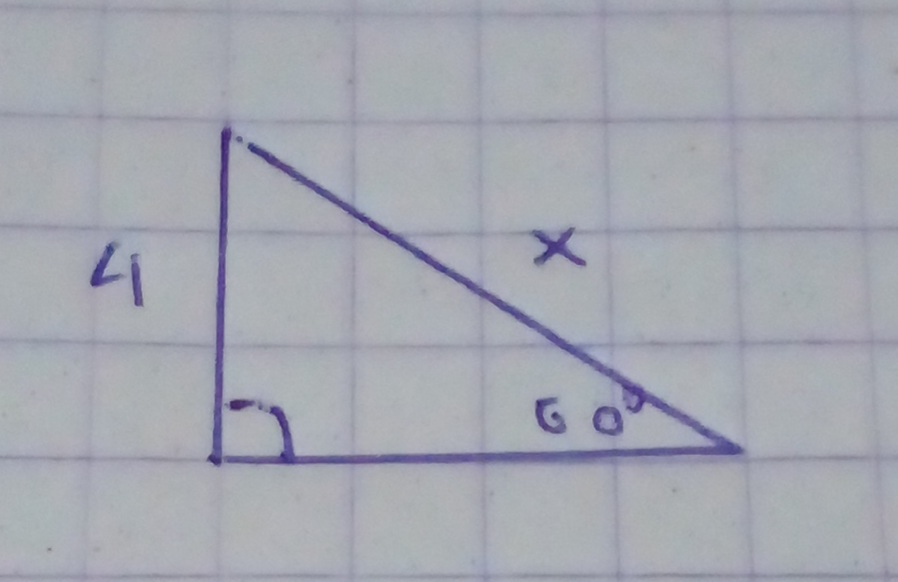
\includegraphics[valign=c,width=50mm,scale=0.5]{seg_19.jpg} \\
\end{center}
\begin{align*}
	\sin{60^{\circ}} &= \frac{o}{h} \\
	\frac{1}{2}\sqrt{3} &= \frac{4}{x} \\
	x &= \frac{4.2}{\sqrt{3}} \\
	x &= \frac{8\sqrt{3}}{3} \\
\end{align*}

\item Jumlah umur Andre dan Sule adalah 42 tahun, sedangkan lima tahun yang akan datang selisih umur mereka adalah 6 tahun. Umur Andre tiga tahun yang lalu adalah\ldots
\options
{19 tahun}
{\textcolor{red}{21 tahun}}
{23 tahun}
{25 tahun}
{27 tahun}
\pemb
Diketahui: \\
\begin{align*}
	A + S &= 42 \\
	(A + 5) - (S + 5) &= 6 \\
\end{align*} Ditanya: \\
A - 3 = ?? \\
Jawab: \\
\begin{center}
\begin{align*}
	S &= 42 - A \\
	\text{Substusi persamaan tersebut ke persamaan ke dua}\\
	(A + 5) - (42 - A + 5) &= 6 \\
	A + 5 - 42 + A - 5 &= 6 \\
	           2A - 42 &= 6 \\
			2A &= 48 \\
			 A &= 24 \\
	\text{Maka umur andre tiga tahun lalu adalah}\\
			 A &= 24 - 3\\
			 A &= 21 \\
\end{align*}
\end{center}

\item Diketahui kubus ABCD.EFGH dengan panjang rusuk 40 cm. Jarak titik A ke perpotongan garis EG dengan HF adalah\ldots
\options
{$30\sqrt{6}$}
{$24\sqrt{6}$}
{$24\sqrt{3}$}
{\textcolor{red}{$20\sqrt{6}$}}
{$20\sqrt{3}$}
\pemb
\begin{center}
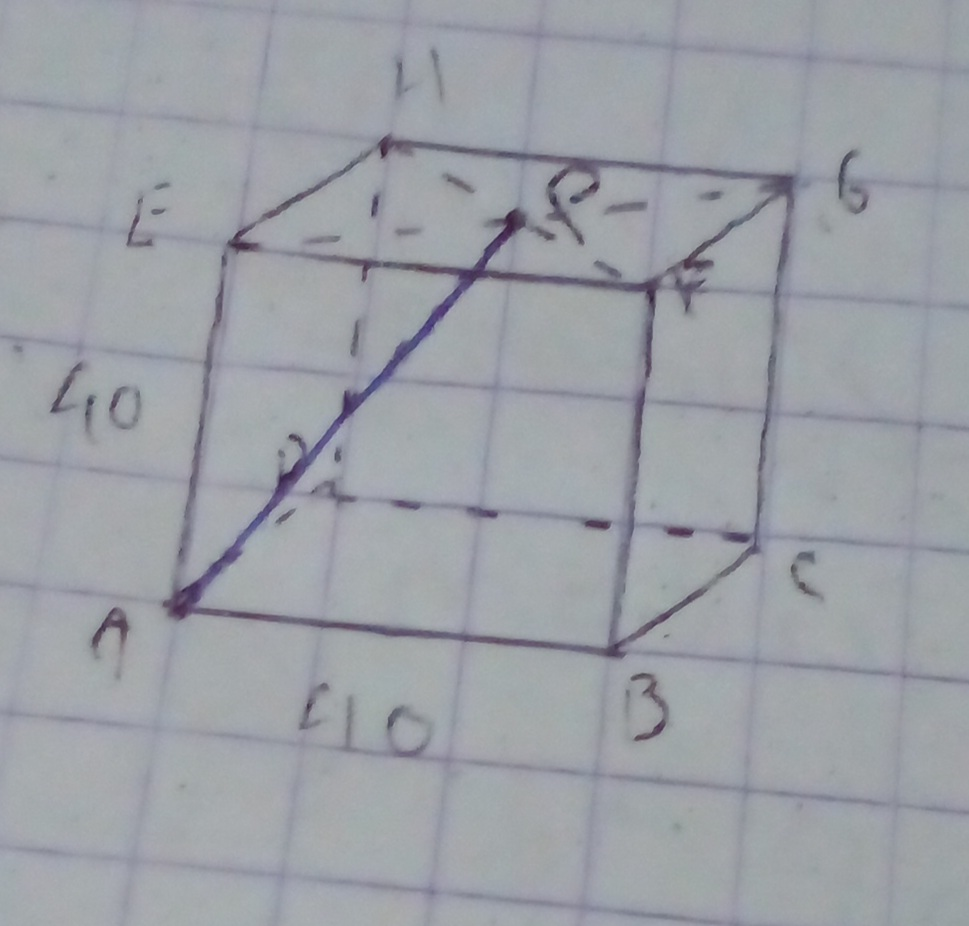
\includegraphics[valign=c,width=50mm,scale=0.5]{cube_21.jpg}\\
Karena EG merupakan diagonal sisi dari persegi EFGH maka 
	\begin{align*}
		EP &= \frac{1}{2} EG \\
		   &= \frac{1}{2} 40\sqrt{2} \\
		   &= 20\sqrt{2} \\
	\end{align*}
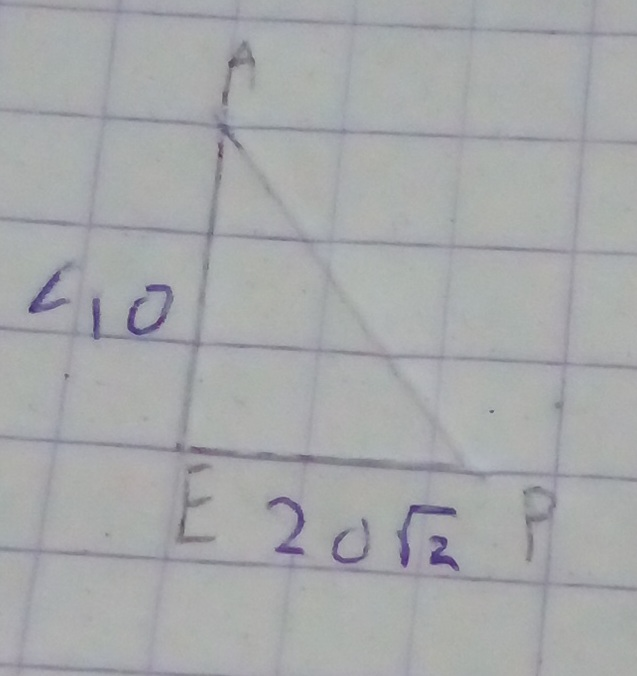
\includegraphics[valign=c,width=50mm,scale=0.5]{seg_21.jpg}\\
\end{center}
\begin{align*}
	AP^2 &= EP^2 + AE^2 \\
	     &= \left(20\sqrt{2}\right)^2 + \left(40\right)^2 \\
	     &= 800 + 1600 \\
	     &= 2400 \\
	  AP &= \sqrt{2400} \\
	     &= 20\sqrt{6} \text{ (D)}
\end{align*}

\item Nilai dari $\lim_{x\to-2}\frac{x^2-x-6}{x+2}$ adalah\ldots
\options
{2}
{1}
{-2}
{-3}
{\textcolor{red}{-5}}
\pemb
\begin{align*}
	\lim_{x\to-2}\frac{x^2-x-6}{x+2} &= \lim_{x\to-2}\frac{\cancel{(x+2)}(x-3)}{\cancel{x+2}} \\
	&= -2 -3 \\
	&= -5 \text{ (E)}
\end{align*}

\item Diketahui $f(x)=4x^3-2x^2+3x+3$. $f'(x)$  merupakan turunan pertama dari $f(x)$. Nilai dari $f'(2)$ adalah\ldots
\options
{36}
{\textcolor{red}{43}}
{61}
{87}
{99}
\pemb
\begin{align*}
	f(x) &= 4x^3-2x^2+3x+3 \\
	f'(x) &= 12x^2-4x+3 \\
	f'(2) &= 12(2)^2-4(2)+3 \\
	      &= 12.4-8+3 \\
	      &= 48-8+3\\
	      &= 43 \text{ (C)}
\end{align*}

\item Turunan pertama fungsi $f(x)=\frac{2x-1}{x+3};x\neq3$ adalah $f'(x)=$\ldots
\options
{\textcolor{red}{$\frac{7}{\left(x+3\right)}$}}
{$\frac{6}{\left(x+3\right)^2}$}
{$\frac{5}{\left(x+3\right)^2}$}
{$\frac{-5}{\left(x+3\right)^2}$}
{$\frac{-7}{\left(x+3\right)^2}$}
\pemb
\begin{align*}
	f(x) &= \frac{2x-1}{x+3} \\
	f'(x) &= \frac{(2)(x+3) - (2x-1)(1)}{(x+3)^2} \\
             &= \frac{2x+6 - 2x+1}{(x+3)^2} \\
             &= \frac{7}{(x+3)^2} \\
\end{align*}

\item Nilai dari integral tak tentu $\int(5x^4-4x^3+x^2-2x+1)dx$ adalah\ldots
\options
{$x^5-x^4+x^3-x+1$}
{$x^5-x^4+x^3-x^2+C$}
{\textcolor{red}{$x^5-x^4+x^3-x^2+x+C$}}
{$20x^3-12x^2+6x-2$}
{$20x^3-12x^2+6x-2+C$}
\pemb
\begin{align*}
	\int(5x^4-4x^3+x^2-2x+1)dx &= x^5-x^4+x^3-x^2+x+C \text{ (C)}
\end{align*}

\item Nilai dari $\int_{-1}^2\left(x^2+x-2\right)dx$ adalah\ldots
\options
{$-3$}
{$-2\frac{1}{2}$}
{\textcolor{red}{$-1\frac{1}{2}$}}
{$1\frac{1}{2}$}
{$3$}
\pemb
\begin{align*}
	\int_{-1}^2\left(x^2+x-2\right)dx 
	&= \left[\frac{1}{3}x^3+\frac{1}{2}x^2-2x\right]_{-1}^2 \\
	&= \left[\frac{2^3}{3}+\frac{2^2}{2}x-2(2)\right]_{-1}^2 - \left[\frac{(-1)^3}{3}x+\frac{(-1)^2}{2}x-2(-1)\right] \\
	&= \left(\frac{16+12-24}{6}\right) - \left(\frac{-2+3+12}{6}\right) \\
	&= \frac{4}{6} - \frac{13}{6} \\
	&= -\frac{9}{6} \\
	&= -\frac{3}{2} \\
	&= -1\frac{1}{2} \text{ (C)}
\end{align*}

\item Luas dareah yang dibatasi kurva $y=x^2-3x-4$ dan sumbu x adalah\ldots
\options
{$-20\frac{5}{6}$}
{$-16\frac{3}{6}$}
{$16\frac{3}{6}$}
{$20\frac{5}{6}$}
{\textcolor{red}{$25\frac{5}{6}$}}
\pemb
\text{Cari titik potong dengan sumbu x}\\
\begin{align*}
	  x^2-3x-4 &= 0 \\
	  (x-4)(x+1) &= 0 \\
	  x = 4 \text{ dan } x = -1
\end{align*}
\begin{align*}
L = -\int_{-1}^4\left(x^2-3x-4\right)dx 
	&= \left[-\frac{1}{3}x^3+\frac{3}{2}x^2+4x\right]_{-1}^4  \\
	&= \left(-\frac{4^3}{3}+\frac{3.4^2}{2}+4.4\right) - \left(-\frac{(1)^3}{3}+\frac{3.(-1)^2}{2}+4.(-1)\right) \\
	&= \left(-\frac{64}{3}+\frac{48}{2}+16\right) - \left(\frac{1}{3}+\frac{3}{2}+(-4)\right) \\
	&= \left(\frac{-128+144+96}{6}\right) - \left(\frac{2+9+(-24)}{6}\right) \\
	&= \left(\frac{112}{6}\right) - \left(\frac{-13}{6}\right) \\
	&= \frac{125}{6} \\
	&= 25\frac{5}{6} \text{ (E)}
\end{align*}

\item Jika lingkaran $x^2+y^2-8x+6y-24=0$ memiliki titik pusat P dan jari-jari r maka\ldots
\options
{P(4,-3) dan r=6}
{\textcolor{red}{P(4,-3) dan r=7}}
{P(4,-3) dan r=8}
{P(-4,3) dan r=7}
{P(-4,3) dan r=8}
\pemb
\begin{align*}
	x^2+y^2-8x+6y-24 &= 0 \\
	x^2+y^2-8x+6y &= 24 \\
	x^2-8x+y^2+6y &= 24 \\
	(x^2-8x+16)+(y^2+6y+9) &= 24+16+9\\
	(x-4)^2+(y+3)^2 &= 49 \\
	\text{Titik pusat} &= (4, -3) \\
	\text{Jari-jari} &= \sqrt{49} = 7 \text{ (B)}
\end{align*}

\item Diketahui titik A=(-2,3) Jika di rotasikan sejauh $90^{\circ}$ berlawanan dengan arah jarum jam dan dilanjutkan dengan refleksi terhadap sumbu x , maka bayangan titik A adalah\ldots
\options
{$A"=(-2,-3)$}
{\textcolor{red}{$A"=(-3,2)$}}
{$A"=(-3,-2)$}
{$A"=(3,-2)$}
{$A"=(3,2)$}
\pemb
Rotasi $90^{\circ}$ berlawanan arah jarum jam\\
$A'=(-3,-2)$ \\
Refleksi terhadap sumbu x \\
$A"=(-3,2)$ (B) \\

\item Titik F (–6, 8) direfleksikan terhadap garis dilanjutkan dengan dilatasi pusat O(0,0) faktor skala 2. Bayangan titik F adalah\ldots
\options
{$F"=(4,-16)$}
{\textcolor{red}{$F"=(-4,16)$}}
{$F"=(-4,-16)$}
{$F"=(-6,-14)$}
{$F"=(-6,14)$}
\pemb
Refleksi terhadap garis x = -4 \\
$F'=(-2,8)$ \\
Refleksi terhadap sumbu x \\
$F"=(-4,16)$ (B) \\

\item Negasi dari pernyataan ”Semua siswa kelas dua belas wajib mengikuti Ujian Nasional Berbasis Komputer dan wajib mengikuti Ujian Sekolah Berstandar Nasional” adalah\ldots
\options
{Ada siswa kelas dua belas tidak wajib mengikuti Ujian Nasional Berbasis Komputer dan tidak wajib mengikuti Ujian Sekolah Berstandar Nasional.}
{\textcolor{red}{Ada siswa kelas dua belas tidak wajib mengikuti Ujian Nasional Berbasis Komputer atau tidak wajib mengikuti Ujian Sekolah Berstandar Nasional.}}
{Ada siswa kelas dua belas tidak wajib mengikuti Ujian Nasional Berbasis Komputer dan wajib mengikuti Ujian Sekolah Berstandar Nasional.}
{Ada siswa kelas dua belas wajib mengikuti Ujian Nasional Berbasis Komputer dan tidak wajib mengikuti Ujian Sekolah Berstandar Nasional.}
{Ada siswa kelas dua belas tidak wajib mengikuti Ujian Nasional Berbasis Komputer
atau wajib mengikuti Ujian Sekolah Berstandar Nasional.}

\item Banyaknya bilangan ratusan yang nilainya lebih dari 400 yang disusun dari angka-angka 1, 2, 3, 4, 5, 6, dan 7 dengan syarat tidak boleh ada angka yang sama adalah\ldots
\options
{90}
{\textcolor{red}{120}}
{126}
{180}
{210}
\pemb
\begin{align*}
	n_{\text{ratusan}}.n_{\text{puluhan}}.n_{\text{satuan}} 
	&= 4.6.5 \\
	&= 120 \text{ (B)}
\end{align*}
Keterangan: \\
4 berasal dari jumlah angka dari daftar yang lebih besar atau sama dengan 4 \\
6 berasal dari jumlah angka dalam daftar dikurangi 1 karena sudah diambil untuk angka ratusan \\
5 berasal dari jumlah angka dalam daftar dikurangi 2 karena sudah diambil untuk angka ratusan dan puluhan \\

\item Pada awal tahun ajaran baru, setiap kelas akan memilih pengurus kelas inti, yaitu ketua, sekretaris dan bendahara kelas.Jika dalam kelas tersebut ada 9 calon pengurus kelas, maka pemilihan 3 pengurus tersebut dapat dilakukan dengan\ldots cara
\options
{60.480}
{3.024}
{514}
{\textcolor{red}{504}}
{84}
\pemb
\begin{align*}
	P_{(9,3)} 
	&= \frac{9!}{(9-3)!} \\
	&= 9.8.7 \\
	&= 504 \text{ (D)}
\end{align*}

\item Sebuah dadu di lempar sebanyak 90 kali. Frekuensi harapan munculnya mata dadu 2 adalah\ldots
\options
{30}
{20}
{\textcolor{red}{15}}
{12}
{10}
\pemb
\[
	\frac{1}{6} \cdot 90=15\text{ (C)}
\]

\item Dua dadu dilempar undi satu kali. Peluang muncul mata dadu 5 pada dadu pertama dan mata dadu 4 pada dadu kedua adalah\ldots
\options
{\textcolor{red}{$\frac{1}{36}$}}
{$\frac{4}{36}$}
{$\frac{11}{36}$}
{$\frac{12}{36}$}
{$\frac{18}{36}$}
\pemb
\[
	\frac{1}{6}.\frac{1}{6} = \frac{1}{36} \text{ (A)}
\]
\item Dari 400 siswa diperoleh data tentang pekerjaan orang tua/ wali. Data tersebut disajikan dalam diagram lingkaran sebagai berikut:\\
	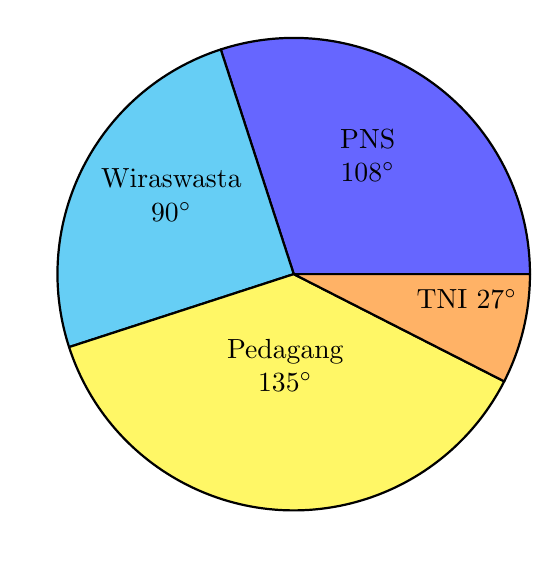
\begin{tikzpicture}
		\pie[sum=auto,text=inside,hide number]{108/PNS \\$108^{\circ}$,
		90/Wiraswasta\\$90^{\circ}$,
		135/Pedagang\\$135^{\circ}$,
		27/TNI $27^{\circ}$ 
		}
	\end{tikzpicture} \\
Berdasarkan data tersebut, pernyataan yang benar adalah....
\options
{Jumlah PNS 12 Orang}
{Jumlah wiraswasta 90 Orang}
{Jumlah pedagang 135 Orang}
{Jumlah TNI/Polri 27 Orang}
{\textcolor{red}{Jumlah TNI/Polri 30 Orang}}
\pemb
\begin{align*}
	\text{PNS} &= \frac{108}{360} \cdot 400 \\
	    &= 120 \\
	\text{Wiraswasta}&= \frac{90}{360} \cdot 400 \\
	    &= 100 \\
	\text{Pedagang} &= \frac{135}{360} \cdot 400 \\
	    &= 150 \\
	\text{TNI / Polri} &= \frac{27}{360} \cdot 400 \\
	    &= 30 \text{ (E)}
\end{align*}

\item Rata-rata nilai ulangan matematika kelas 12 Bismen adalah 85. Jika nilai tersebut di pisahkan antara kelompok siswa laki-laki dan siswa perempuan, akan diperoleh rata-rata nilai siswa laki-laki sebesar 83 dan rata-rata siswa perempuan sebesar 88. Perbandingan antara banyak siswa laki-laki dan siswa perempuan adalah\ldots
\options
{2:3}
{3:5}
{5:3}
{5:2}
{\textcolor{red}{3:2}}
\pemb
Diketahui: \\
\begin{align*}
	\text{Rata-rata laki-laki} = \bar{x_{l}} &= 83 \\
	\text{Rata-rata perempuan} = \bar{x_{p}} &= 88 \\
	\text{Rata-rata keseluruhan} = \bar{x} &= 85
\end{align*}
Ditanya: \\
Perbandingan banyak siswa laki-laki dan perempuan \\
Jawab: \\
Misal:
\begin{align*}
	\text{Jumlah siswa} &= A \\
	\text{Jumlah siswa laki-laki} &= L \\
	\text{Jumlah siswa perempuan} = P &= A-L \\
\end{align*}
Maka
\begin{align*}
	83L+88(A-L)&=85A\\
	83L+88A-88L&=85A\\
	83L-88L&=85A-88A\\
	-5L&=-3A\\
	L&=\frac{3}{5}A \\
	P&=\frac{2}{5}A \\
	L:P&=3:2 \text{ (C)}
\end{align*}

\item Perhatikan tabel distribusi frekuensi di bawah ! \\
\\
\begin{center}
\begin{tabular}{|c|c|}
	\hline
	Tinggi & Frekuensi \\
	\hline
	33-36 & 2 \\
	\hline
	37-41 & 9 \\
	\hline
	42-46 & 12 \\
	\hline
	47-51 & 15 \\
	\hline
	52-56 & 8 \\
	\hline
	57-61 & 4 \\
	\hline
\end{tabular}
\end{center}
Modus dari data tersebut adalah\ldots \\
\options
{47.0}
{47.5}
{\textcolor{red}{48.0}}
{48.5}
{49.0}
\pemb
\begin{align*}
	Mo&=Tb\left(\frac{d_{1}}{d_{1}+d_{2}}\right)p\\
	%Tb&=46.5\\
	%d_{1}
	%&=15-12 \\
	%&=3
	%d_{2}
	%&=15-8 \\
	%&=7
	%p&=5\\
	Mo&=46.5+\left(\frac{3}{3+7}\right)5\\
	&=46.5+1.5\\
	&=48.0\text{ (C)}
\end{align*}

\item Simpangan baku dari data 12, 14, 15, 14, dan 10 adalah\ldots
\options
{\textcolor{red}{$\frac{4\sqrt{5}}{5}$}}
{$\frac{4\sqrt{3}}{5}$}
{$\frac{4}{5}$}
{$\frac{1\sqrt{5}}{5}$}
{$\frac{1\sqrt{3}}{5}$}
\pemb
\begin{align*}
  S_{B} &=\sqrt{\frac{1}{n}\sum\left(\bar{x}-x\right)^2}\\
\bar{x} &=\frac{12+14+15+14+10}{5}\\
	&=\frac{65}{5}\\ &=13\\
  S_{B} &=\sqrt{\frac{1}{5}(1+1+4+1+9)}\\
	&=\sqrt{\frac{16}{5}} \\
	&=\frac{\sqrt{16}}{\sqrt{5}} \\
	&=\frac{4}{\sqrt{5}} \cdot \frac{\sqrt{5}}{\sqrt{5}} \\
	&=\frac{4\sqrt{5}}{5} \text{ (A)}
\end{align*}

\item Perhatikan tabel dibawah ini\\
\begin{center}
\begin{tabular}{|l|c|c|c|c|c|c|}
	\hline
	Nilai & 6 & 7 & 8 & 9 & 10 & 12 \\
	\hline
	Frekuensi & 5 & 8 & 12 & 14 & 6 & 5 \\
	\hline
\end{tabular}
\end{center}
Simpangan Kuartil tabel di atas adalah\ldots
\options
{14}
{12}
{8}
{6}
{3}
\pemb
\begin{align*}
	Q_{d}&=\frac{1}{2}(Q_3-Q_1) \\
	Q_{3}
	&=\frac{x_{\left(\lfloor \frac{3.50}{4} \rfloor \right)}+x_{\left( \lfloor \frac{3.50}{4} \rfloor +1\right)}}{2}\\
	&=\frac{x_{(37)}+x_{(38)}}{2}\\
	&=\frac{9+9}{2}\\
	&=9\\
	Q_{1}
	&=\frac{x_{\left(\lfloor \frac{50}{4} \rfloor \right)}+x_{\left(\lfloor \frac{50}{4} \rfloor +1\right)}}{2}\\
	&=\frac{x_{(12)}+x_{(13)}}{2}\\
	&=\frac{7+7}{2}\\
	&=7\\
	Q_d&=\frac{9-7}{2}\\&=1
\end{align*}

	


\end{enumerate}
\end{document}
